\subsection*{Задание}

\begin{enumerate}
\item Реализуйте программный продукт на языке Python, используя регулярные выражения по варианту, представленному в таблице.
\item Для своей программы придумайте минимум 5 тестов. Каждый тест является отдельной сущностью, передаваемой регулярному выражению для обработки. Для каждого теста необходимо самостоятельно (без использования регулярных выражений) найти правильный ответ. После чего сравнить ответ, выданный программой, и полученный самостоятельно. Все 5 тестов необходимо показать при защите. Пример тестов приведён в таблице.
\item Можно использовать циклы и условия, но основной частью решения должны быть регулярные выражения.
\end{enumerate}

\begin{figure}[h]
	\centering
	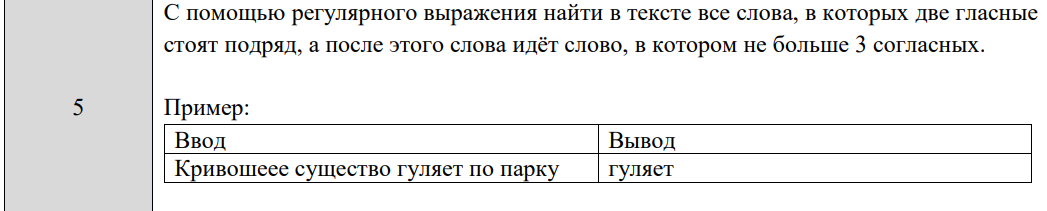
\includegraphics[scale=0.7]{task_2}
\end{figure}

\subsection*{Тестовые файлы}
\subsubsection*{Тест 1}
\textit{Кривошеее существо гуляет по парку}

\subsubsection*{Тест 2}
\textit{Кривоногое создание с интересом рассматривало яркое солнце над горизонтом}

\subsubsection*{Тест 3}
\textit{Синее небо раскрылось перед маленьким озером, окруженным камнями. Двуххвостое животное лениво отдыхало под тихим ветром на берегу моря.}

\subsubsection*{Тест 4}
\textit{Безухое создание медленно пробиралось через тёплую траву на поляне.}

\subsubsection*{Тест 5}
\textit{Пятиногое создание медленно двигалось через зелёную поляну у леса.}

\subsection*{Листинг}
\begin{minted}[breaklines]{python}
import re
from pathlib import Path

TEXTS_PATH = Path(__file__).parent / "texts" / "task_2"
PATTERN = re.compile(
    r"\b\w*[аеёиоуыэюя]{2}\w*\b(?!\s+(?:[аеёиоуыэюя]*[бвгджзйклмнпрстфхцчшщ]){4,})",
    flags=re.MULTILINE
)
CORRECT_ANSWERS = (
    {"гуляет"},
    {"создание"},
    {"Синее", "животное"},
    {"тёплую"},
    {"зелёную"}
)


def find_words(text: str) -> set[str]:
    return set(PATTERN.findall(text))


def main() -> None:
    for i in range(1, 6):
    text = (TEXTS_PATH / f"text_{i}").read_text(encoding="utf-8")
    words = find_words(text)

    if words != CORRECT_ANSWERS[i - 1]:
        print(
            f"Ошибка в тесте {i}. "
            f"Ожидалось - {CORRECT_ANSWERS[i - 1]}, "
            f"Результат - {words}"
        )
    else:
        print(f"Текст {i}: слова - {words}")
    print("=" * 100)


if __name__ == '__main__':
    main()
\end{minted}

